%% LyX 2.1.0 created this file.  For more info, see http://www.lyx.org/.
%% Do not edit unless you really know what you are doing.
\documentclass[12pt,spanish]{article}
\usepackage[LGR,T1]{fontenc}
\usepackage[latin9]{inputenc}
\usepackage{geometry}
\geometry{verbose,tmargin=3cm,bmargin=2cm,lmargin=3cm,rmargin=2cm}
\setlength{\parskip}{\medskipamount}
\setlength{\parindent}{0pt}
\usepackage{float}
\usepackage{textcomp}
\usepackage{amsmath}
\usepackage{graphicx}
\usepackage{setspace}
\usepackage[authoryear]{natbib}
\onehalfspacing

\makeatletter

%%%%%%%%%%%%%%%%%%%%%%%%%%%%%% LyX specific LaTeX commands.
\DeclareRobustCommand{\greektext}{%
  \fontencoding{LGR}\selectfont\def\encodingdefault{LGR}}
\DeclareRobustCommand{\textgreek}[1]{\leavevmode{\greektext #1}}
\DeclareFontEncoding{LGR}{}{}
\DeclareTextSymbol{\~}{LGR}{126}

%%%%%%%%%%%%%%%%%%%%%%%%%%%%%% User specified LaTeX commands.
 \usepackage[colorlinks=true, citecolor=black, linkcolor=black, urlcolor=black]{hyperref}

\makeatother

\usepackage{babel}
\addto\shorthandsspanish{\spanishdeactivate{~<>}}

\begin{document}
\noindent \begin{center}
{\large{}\renewcommand{\thepage}{\Roman{page}} \setcounter{page}{1}
\pagenumbering{Roman}}
\par\end{center}{\large \par}

\noindent \begin{center}
EVALUACI�N DE MODELOS DE APRENDIZAJE ESTAD�STICO APLICADOS EN ESTIMACI�N
DE VARIABLES BIOF�SICAS EN CULTIVOS DE CA�A DE AZ�CAR \vspace{1cm}

\par\end{center}

\noindent \begin{center}
Proyecto de Maestr�a\\
\vspace{0.7cm}

\par\end{center}

\noindent \begin{center}
\includegraphics[scale=0.3]{\string"../Figures/LOGO UBA\string".jpg}
\par\end{center}

\noindent \begin{center}
CAMILO ALBERTO HERRERA ROZO
\par\end{center}

\vspace{0.7cm}


\noindent \begin{center}
Director\\
PABLO A. CIPRIOTTI\\
Ingeniero Agr�nomo - Dr. Ciencias Agropecuarias
\par\end{center}

\vspace{0.7cm}


\noindent \begin{center}
\vspace{0.7cm}

\par\end{center}

\noindent \begin{center}
UNIVERSIDAD DE BUENOS AIRES\\
FACULTAD DE AGRONOMIA\\
MAESTR�A EN BIOMETR�A Y MEJORAMIENTO\\
Buenos Aires - Argentina, Junio \\
2014
\par\end{center}

\pagebreak{}

\renewcommand{\thepage}{\arabic{page}} \setcounter{page}{1}


\section*{{\normalsize{}Introducci�n}}

La Agricultura de precisi�n y manejo sitio-espec�fico (AEPS), se define
como el arte de realizar las pr�cticas agron�micas requeridas por
una especie vegetal, de acuerdo con las condiciones espaciales y temporales
del sitio donde se cultiva, para obtener de ellas su rendimiento potencial
\citep{Sandoval2012}. La medici�n de variables biof�sicas como lo
son �rea foliar (AF) o �ndices de �rea foliar (IAF) en cultivos de
ca�a de az�car se realiza en la actualidad por medio de procesos destructivos.
Tambi�n realizar el conteo de cantidad de tallos (NT) en cultivos
de ca�a de az�car es un proceso de estimaci�n emp�rico y poco preciso,
estas dos caracter�sticas plantean un panorama interesante de investigaci�n
con la finalidad de lograr generar nuevos m�todos de estimaci�n indirecta
y precisa, a los cuales la estad�stica pueden ser una ayuda invaluable.

En tal sentido, existen actualmente una gran cantidad de m�todos estad�sticos
que permiten realizar infinidad de an�lisis distintos y cubrir cualquier
variable y aplicaci�n. El uso de la inteligencia artificial (visi�n
computacional, sistemas expertos, sistemas de ayuda de decisi�n, etc.)
y otras t�cnicas prometedoras de esta (redes neuronales, l�gica difusa
y bioinform�tica) pueden proporcionar soluciones a los problemas anal�ticos
en sistemas agr�colas complejos de manera eficaz \citep{M.2005}.
En este contexto, para analizar estructuras de datos como los que
se mencionan en el p�rrafo anterior, tres m�todos son de particular
inter�s. Se desea evaluar el funcionamiento, la adaptaci�n, la eficiencia
y la precisi�n de los mismos, ya que son herramientas potencialmente
importantes de aplicar en casos de aprendizaje y clasificaci�n estad�stica
\citep{Mitchell:1997:ML:541177}\citep{citeulike:1720151}, Las metodolog�as
son: PLS o Regresi�n por m�nimos cuadrados parciales \citep{CEM:CEM1180040607},
Random Forest \citep{Breiman2001} y el Aprendizaje por cuantificaci�n
vectorial (LVQ) \citep{Kohonen:1997:SM:261082}. Estos tres m�todos
ser�n aplicados a im�genes multiespectrales \citep{hough1991satellite}
y datos obtenidos mediante procesos de simulaci�n del comportamiento
de cultivos de ca�a de az�car.

En este proyecto de tesis se pretende integrar m�todos estad�sticos
y sistemas de visi�n artificial o visi�n por computadora\citep{gonzalez1996tratamiento},
para mejorar la comprensi�n de procesos naturales que ocurren en los
cultivos. Dichos procesos son captados por sensores remotos, y revelan
patrones espaciales presentes en los cultivos \citep{Gutierrez2006}.
Adicionalmente se desea cubrir la necesidad cada vez mayor de automatizar
y mejorar procesos costosos o de caracter�sticas destructivas relacionados
a la toma de informaci�n, permitiendo hacer un mejor manejo agron�mico
y apuntando a sistemas de agricultura de precisi�n y manejo sitio-espec�fico
en cultivos de ca�a de az�car. Consecuentemente, el objetivo general
de este proyecto es el de integrar m�todos estad�sticos y sistemas
de visi�n artificial o visi�n por computador, para mejorar la comprensi�n
de procesos naturales, reflejados por cultivos de ca�a de az�car y
captados por sensores remotos. Son objetivos espec�ficos los siguientes:
\begin{itemize}
\item Evaluar el funcionamiento, adaptaci�n, eficiencia y precisi�n de tres
algoritmos de inteligencia artificial {[}Aprendizaje por cuantificaci�n
vectorial (LVQ){]}, {[}La Regresi�n por m�nimos cuadrados Parciales{]}
y {[}Random Forest{]} aplicados en imagenes multiespectrales de cultivos
de ca�a de az�car.
\item Estimar el �rea foliar (AF) y el �ndice de �rea foliar (IAF) en cultivos
de ca�a de az�car y la cantidad de tallos (NT) en cultivos de ca�a
de az�car.
\item Ajustar modelos estad�sticos y de inteligencia artificial que relacionen
correctamente la informaci�n de las im�genes multiespectrales a las
variables de cultivo (AF), (IAF) y (NT).
\end{itemize}

\section*{{\normalsize{}Revisi�n literaria}}

La ca�a de az�car (Saccharum officinarum) es un cultivo de zonas tropicales
y subtropicales que se propaga mediante la plantaci�n de trozos y/o
v�stagos de ca�a, donde de cada nudo sale una planta nueva e id�ntica
a la original. Existe una infinidad de m�todos relacionados con la
medici�n del desarrollo de los cultivos entre estos m�todos encontramos
nuevas aplicaciones como lo son la percepci�n remota o teledetecci�n,
la cual se define como el grupo de t�cnicas para la obtenci�n de informaci�n
confiable sobre las propiedades f�sicas de ciertas superficies u objetos
y su entorno, desde distancias relativamente grandes, sin contacto
f�sico con ellos \citep{GEO:4427856}. Las im�genes adquiridas por
sensores en plataformas a�reas o satelitales en el mundo agropecuario
tienen un potencial que se ha venido explorando con mayor �nfasis
en la �ltima d�cada \citep{Gutierrez2006}. 

El IAF es el �rea ocupada por hojas verdes en relaci�n con la unidad
de superficie de suelo. La informaci�n precisa y oportuna sobre IAF
tiene gran importancia y aplicaciones en la agricultura para la estimaci�n
del rendimiento y la evaluaci�n del estr�s en los cultivos, y en la
ecolog�a para el estudio de la producci�n primaria y el cambio ambiental
\citep{Curran1983}. Las principales aplicaciones de las t�cnicas
de teledetecci�n est�n dentro de los campos de la inteligencia agr�cola,
la gesti�n agr�cola y la investigaci�n ecol�gica \citep{Curran1983}.
Desde los inicios de la percepci�n remota los �ndices espectrales
de vegetaci�n han sido �tiles y f�ciles de calcular para relacionarlos
con diversas variables agron�micas. Aunque los �ndices espectrales
de vegetaci�n en muchos casos muestran excelentes relaciones con estas
variables, es necesario calibrar o comprender la equivalencia de sus
valores en la estimaci�n de contenidos de clorofila, IAF o biomasa
\citep{Sandoval2012}.

 Hoy en d�a existen muchas t�cnicas estad�sticas que el agricultor
puede aprovechar para la estimaci�n de variables del cultivo, entre
estas est� el aprendizaje autom�tico que es una rama de la Inteligencia
Artificial (IA) cuyo objetivo es desarrollar t�cnicas que permitan
a las computadoras aprender. Una m�quina es un sistema organizado
capaz de transformar un cierto mensaje de entrada en otro de salida,
de acuerdo con alg�n principio de transformaci�n. Si tal principio
est� sujeto a cierto criterio de validez de funcionamiento, y si el
m�todo de transformaci�n se ajusta a fin de que tienda a mejorar el
funcionamiento del sistema de acuerdo con este criterio, se dice que
el sistema aprende. 

\citep{citeulike:1720151} define las m�quinas de aprendizaje o el
aprendizaje autom�tico como el campo de estudio que da a las computadoras
la capacidad de aprender sin estar programado expl�citamente, lo cual
ser�a un gran avance en las t�cnicas de estimaci�n en cultivos de
ca�a de az�car, sobre todo cuando la informaci�n proviene de im�genes
digitales, lo cual genera un flujo grande de informaci�n generando
la necesidad de realizar el an�lisis de grandes bases de datos, el
cual requiere m�todos estad�sticos capaces de tratar con estructuras
de datos multivariados y no lineales, herramientas matem�ticas basadas
en la miner�a de datos proporcionan un marco adecuado para la extracci�n
de informaci�n �til a partir de grandes bases de datos, as� como tambi�n
pueden conducir al descubrimiento de conocimiento \citep{Ferraro2008}. 

La regresi�n por m�nimos cuadrados parciales o PLS, el algoritmo de
random forest o arboles aleatorios y el aprendizaje por cuantificaci�n
vectorial (LVQ) son tres metodolog�as de mucho inter�s para el desarrollo
de esta investigaci�n ya que aunque son m�todos cada uno desarrollado
para diferentes aplicaciones en un principio son altamente escalables
y se espera obtener resultados interesantes con la aplicaci�n de m�todos
que con anterioridad no se han probado sobre cultivos de ca�a.


\subsubsection*{PLS o Regresi�n por m�nimos cuadrados parciales: }

La Regresi�n por m�nimos cuadrados se introdujo hace casi treinta
a�os y ha tenido un gran desarrollo en �reas como la Quimiometr�a,
donde se analizan datos que se caracterizan por muchas variables predictoras,
con problemas de multicolinealidad, y pocas unidades experimentales
en estudio (\citet{Geladi19861} , \citet{CEM:CEM1180040607}).

Es una particular forma de an�lisis multivariante, este m�todo relacionado
con la regresi�n de componentes principales, PCR (\textquotedblleft Principal
components regression\textquotedblright ) posee valiosas ventajas
te�ricas y computacionales que han llevado a innumerables aplicaciones.
PLS se utiliza para encontrar las relaciones fundamentales entre dos
matrices (X e Y), es decir, un enfoque de variable latente para el
modelado de las estructuras de co varianza en estos dos espacios.

Un modelo de PLS trata de encontrar el sentido multidimensional en
el espacio X que explica la direcci�n de la m�xima varianza multidimensional
en el espacio Y \citep{Tenenhaus2005}. Estos m�todos tienen ventajas
intr�nsecas cuando se le compara con m�todos univariados, Todas las
variables relevantes son incluidas en el modelo PLS. La suposici�n
b�sica de todos estos modelos es que el sistema o proceso estudiado
depende de un n�mero peque�o de variables latentes (V.L.). Este concepto
es similar al de componentes principales. Las variables latentes son
estimadas como combinaciones lineales de las variables observadas.


\subsubsection*{Random Forest o �rboles Aleatorios: }

En una serie de documentos e informes t�cnicos, Breiman (\citet{Breiman1996},
\citet{Breim2000}, \citet{Breiman2001}, \citet{Breim2004}) demostraron
que hay ganancias sustanciales en la clasificaci�n y la exactitud
de la regresi�n y se puede lograr mediante el uso de conjuntos de
�rboles, donde de acuerdo con un par�metro de azar crece cada �rbol
en cada conjunto de �rboles. Las predicciones finales se obtienen
de las agregaciones sobre el conjunto de datos. Como los componentes
de base del conjunto son predictores con estructura de �rbol, y desde
cada uno de estos �rboles se construye utilizando una inyecci�n de
aleatoriedad, estos procedimientos son llamados \textquotedbl{}Random
Forest\textquotedbl{}.

El random Forest es una combinaci�n de �rboles predictores tal que
cada �rbol depende de los valores de un vector aleatorio probado independientemente
y con la misma distribuci�n para cada uno de �stos. Es una modificaci�n
sustancial de bagging que construye una larga colecci�n de �rboles
no correlacionados y luego los promedia. Random Forest es una uni�n
entre m�todos de clasificaci�n y m�todos de regresi�n, esta opera
por la construcci�n de una multitud de �rboles de decisi�n en el entrenamiento
y en la salida una clase el cual es el modo de salida de los �rboles
individuales. 


\subsubsection*{Aprendizaje por cuantificaci�n vectorial (LVQ):}

LVQ se puede entender como un caso especial de una red neuronal artificial,
con mayor precisi�n, este aplica el concepto de ({[}winner-take-all{]}
el ganador toma todo mediante el aprendizaje de Hebb) . Es un precursor
de los mapas auto-organizados (SOM) y est� relacionado con el algoritmo
de gas neural y con el algoritmo de K vecinos m�s cercanos (k-NN).

El aprendizaje por cuantificaci�n vectorial (LVQ) supone una extensi�n
del aprendizaje competitivo donde los prototipos est�n etiquetados.
Ahora, adem�s de considerar la cercan�a de un prototipo se puede evaluar
la clase de �ste e imponer, por lo tanto, correcciones de premio (acercamiento)
o castigo (alejamiento). En ciencias de la computaci�n, aprendizaje
cuantificaci�n vectorial (LVQ), est� basado en prototipos de algoritmos
de clasificaci�n supervisada. LVQ es la contraparte supervisada de
los sistemas de cuantificaci�n vectorial \citep{hastie_09_elements-of.statistical-learning}. 


\subsubsection*{Validaci�n cruzada}

Probablemente el m�s simple y ampliamente usado m�todo para estimar
el error en predicci�n es la validaci�n cruzada, este m�todo estima
directamente el error esperado de una muestra-extra $Err=E\left[L\left(Y,\hat{f}\left(X\right)\right)\right]$,
el error medio generalizado cuando el m�todo $\hat{f}\left(X\right)$,
se aplica a una muestra de prueba independiente de la distribuci�n
conjunta de X e Y. Como se mencion� anteriormente, podr�amos esperar
que la validaci�n cruzada estima el error condicional, con el conjunto
de entrenamiento $\tau$ el cual se mantiene fijo.


\paragraph{Validaci�n cruzada K-Fold}

Lo ideal ser�a que si tuvi�ramos suficientes datos, as� tendr�amos
que dejar de lado un conjunto de validaci�n y se utiliza para evaluar
el desempe�o de nuestro modelo de predicci�n. Puesto que los datos
a menudo son escasos, esto no suele ser posible. A la delicadeza del
problema, la validaci�n cruzada K veces utiliza parte de los datos
disponibles para ajustar el modelo, y una parte distinta para comprobarlo.
Donde dividimos los datos en K partes m�s o menos del mismo tama�o;
Por ejemplo, cuando $K=5$, el escenarios seria as� :

\begin{figure}[H]
\begin{centering}
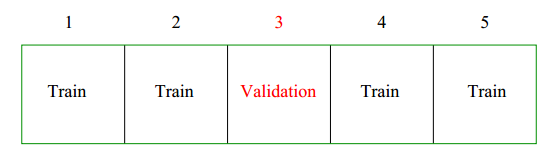
\includegraphics[scale=0.5]{C:/Users/SAMSUNG/Documents/GitHub/ProyectoMaestria/imagenes/kfold}
\par\end{centering}

\centering{}\protect\caption{k-fold}
\end{figure}


Para la parte de orden k (k=3), nos ajustamos el modelo a la otra
K - 1 parte de los datos, y se calcula el error de predicci�n del
modelo ajustado la k-th para predecir la parte de orden k de los datos.
Hacemos esto para k = 1, 2,. . . , K y se combinan las estimaciones
del error de predicci�n de K.

Suponga \textgreek{k} : \{1,. . . , N\} \textrightarrow{} \{1,. .
. , K\} una funci�n de indexaci�n que indica la partici�n a la que
la observaci�n i es asignada por la aleatorizaci�n. Denotemos por
$\hat{f}^{-k}\left(X\right)$ � la funci�n de m�dulos, calculado con
la parte de orden k de los datos eliminados. A continuaci�n, la estimaci�n
de la validaci�n cruzada de error de predicci�n es:

\[
CV\left(\hat{f}\right)=\frac{1}{N}\overset{N}{\underset{i=1}{\sum}L\left(y_{i},\hat{f}^{-k\left(i\right)}\left(x_{i}\right)\right)}
\]


La t�pica elecci�n para k es 5 o 10, pero incluso podr�amos tener
una elecci�n de K=N lo que es conocido como una validaci�n cruzada
\textquotedblleft leave-one-out \textquotedblright{} donde el estimador
de validaci�n cruzada es aproximadamente insesgado, pero no se utiliza
mucho este caso ya que cuando tenemos tantos conjuntos de validaci�n,
existen muchos conjuntos casi iguales, por esta raz�n en la mayor�a
de las veces de opta por selecci�n de un K un poco m�s conservador
como lo es 5 o 10 lo que es suficiente para obtener buenos resultados
\citep{hastie_09_elements-of.statistical-learning}.


\subsection*{{\normalsize{}Antecedentes}}

Hace m�s de 50 a�os se realiza la toma de fotograf�as a color e infrarrojo
para seguir el crecimiento de las plantas como se puede observar en
\citet{Colwell1956}. En la actualidad, estos m�todos est�n siendo
reevaluados para realizar an�lisis dentro de la variabilidad espacial
en la agricultura de precisi�n, ya que las im�genes a�reas se pueden
adquirir r�pidamente durante los per�odos cr�ticos del crecimiento
r�pido de las plantas \citep{Blackmer1996}.

A nivel mundial pa�ses como Francia y Brasil han realizado trabajos
para estimar algunos par�metros biof�sicos e inclusive para pronosticar
la producci�n de ca�a de az�car. En Francia \citet{Begue2008} haciendo
uso del �ndice de vegetaci�n normalizado (NDVI) en cultivos de variabilidad
espacial (independiente a las etapas de crecimiento de los cultivos),
demostraron que en una escala estacional, el patr�n de crecimiento
dentro de un campo depende de la etapa fenol�gica del cultivo, a escala
anual los mapas NDVI revelaron patrones estables. Lo anterior permite
concluir que es necesario conocer el ciclo de crecimiento del cultivo
para interpretar correctamente los patrones espaciales. Las im�genes
de una fecha �nica pueden ser insuficientes para el diagn�stico de
la situaci�n de los cultivos o para aplicaciones en predicci�n.

En \citet{H.S.Sandhu2012} se evaluaron las calificaciones visuales
subjetivas de crecimiento del cultivo de la ca�a de az�car para la
estimaci�n de par�metros de rendimiento del cultivo y paralelamente
se realizaron mediciones de los IAF, donde se encontr� que existe
relaciones importantes entre estos sistemas de evaluaci�n visual,
los �ndices IAF y la estimaci�n de la poblaci�n, pero estas relaciones
son v�lidas solo en algunos estados del crecimiento del cultivo, por
lo tanto las estimaciones no eran buenas fuera de algunos periodos
del desarrollo del cultivo, sobre todo en las primeras etapas del
crecimiento, lo que impide tomar decisiones tempranas respecto al
manejo del cultivo.

En Brasil \citet{Almeida2006} propone un m�todo para realizar predicci�n
del rendimiento sobre cultivos de ca�a de az�car usando �ndices de
vegetaci�n espectral, mediante an�lisis de componentes principales
e informaci�n hist�rica de los cultivos. Para este estudio se utilizaron
im�genes (ETM +) / Landsat-7 e im�genes ASTER/Terra. Este m�todo presentado
comprende varias etapas que finalmente e logra una s�ntesis de toda
la informaci�n tanto de la imagen como de la informaci�n hist�rica
permitiendo la normalizaci�n de todas las variables en conjunto, haciendo
posible expresar todos los datos en im�genes s�ntesis.

Sud�frica es el l�der en producci�n de ca�a de az�car en �frica y
uno de los m�s grandes productores en el mundo, El monitoreo de estos
factores de estr�s del cultivo de ca�a es de vital importancia para
tomar acciones preventivas y de mitigaci�n sobre el cultivo. \citet{abdel2010potential}
explor� el potencial de usar sensores remotos en cultivos de ca�a
de az�car, mediante el uso de im�genes Lansat TM y ETM+ con las cuales
gener� modelos de predicci�n de rendimiento de ca�a aplicando algoritmos
de random forest optimizados, logrando una estimaci�n bastante buena
para algunas de las variedades estudiadas.







\section*{{\normalsize{}Metodolog�a}}

En el desarrollo de este proyecto de investigaci�n se cuenta con 2
escenarios a desarrollar sobre este cultivo, donde una parte del estudio
se realizara en cultivos experimentales y la otra parte del estudio
se realizar� sobre cultivos de ca�a comerciales, cada uno de estos
cultivos se encuentran ubicados en el valle geogr�fico del r�o Cauca. 

Los cultivos experimentales se utilizar�n inicialmente por la necesidad
de realizar pruebas sobre cultivos donde se puedan controlar las distintas
fuentes de variaci�n como lo son el sistemas de riego, el tama�o del
lote productivo, la fecha y densidad de siembra, el manejo del suelo,
el seguimiento del cultivo durante el crecimiento, y su fertilizaci�n,
entre otros factores que en un cultivo comercial no es posible. As�,
se limitar� la variabilidad para realizar una correcta calibraci�n
y aproximaci�n de las variables a estimar. Estos cultivos son campos
de investigaci�n de Cenica�a que han sido designados para este fin.
Los cultivos comerciales ser�n un objetivo estrat�gico a evaluar,
pues al depender de las pol�ticas de plantaci�n de los ingenios, no
es posible controlar muchos de los factores relacionados con el crecimiento
del cultivo.

Estos dos escenarios involucrados poseen unas caracter�sticas espec�ficas
como el tipo de suelo en el que se encuentran, adem�s de las caracter�sticas
clim�ticas e inclusive en muchos casos se tienen registros hist�ricos
de su producci�n. Respecto a los tipos de suelos y caracter�sticas
del �rea de estudio, los cultivos evaluados estar�n sobre �reas agroecol�gicas
catalogadas como\textbf{ 6H1 }(Suelos de texturas finas y contenidos
de arcilla entre 35\% y 60\%, moderadamente bien drenados que poseen
caracter�sticas de permeabilidad baja <200 mm/a�o) �rea predominante
en el Valle del Cauca, de acuerdo a clasificaci�n presentada en \citealp{CarbonellG.2001}
 y se evaluar�n las variedades gen�ticas de ca�a CC-8592 y CC-934418,
las cuales son de gran inter�s de estudio para el centro de investigaci�n.

Una vez realizadas las pruebas de estimaci�n sobre los cultivos experimentales,
se tendr� una metodolog�a definida para la estimaci�n de las variables
biof�sicas y del tama�o la poblaci�n del cultivo partir de im�genes
multiespectrales de alta resoluci�n. Posteriormente, los cultivos
comerciales servir�n para realizar la validaci�n del m�todo desarrollado
inicialmente con los cultivos experimentales.

El procedimiento de toma de informaci�n se realizar� mediante aviones
ultra-livianos de fumigaci�n del cultivo con una c�mara multi-espectral
\footnote{http://www.tetracam.com/Products-Mini\_MCA.htm%
} (Figura: \ref{fig:Camara-Multiespectral} ) para toma de im�genes
en campo enlazada a sistemas de GPS, que permitir�n una mejor geolocalizaci�n
de las tomas (im�genes) realizadas.

\begin{figure}[H]
\begin{centering}
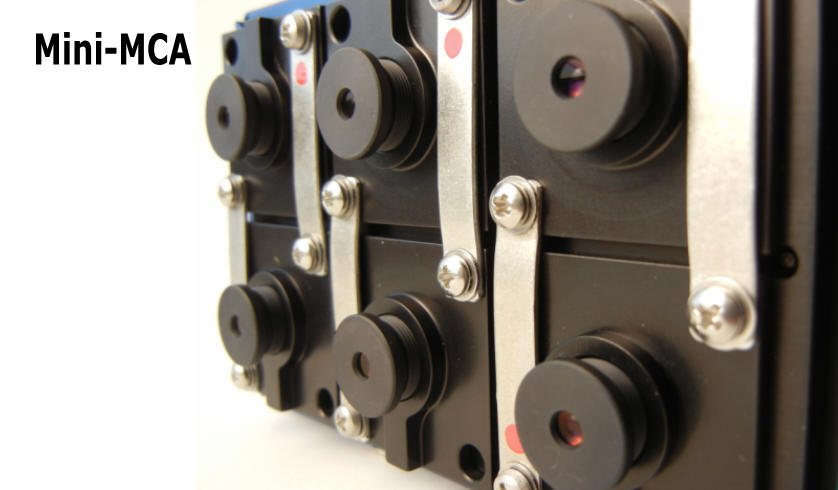
\includegraphics[width=0.4\paperwidth,height=0.15\textheight]{../Figures/tetracam}
\par\end{centering}

\protect\caption{C�mara Multi-espectral \label{fig:Camara-Multiespectral} }
\end{figure}


Se estudiar� la informaci�n reflectada por el cultivo mediante im�genes
multiespectrales en formato raster (imagen matricial), donde la informaci�n
de cada imagen se considera como una matriz de datos de dimensiones
(n x m), siendo n el n�mero de p�xel verticales y m el n�mero de p�xel
horizontales. Estas dimensiones est�n determinadas por la resoluci�n
de la c�mara mediante la cual se realiza la toma de la informaci�n.
Adem�s en este caso al tratarse de im�genes multiespectrales cada
imagen cuenta con 6 bandas espectrales las cuales corresponden a un
rango del espectro.

\begin{figure}[H]
\begin{centering}
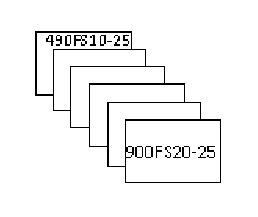
\includegraphics{../Figures/bandas2}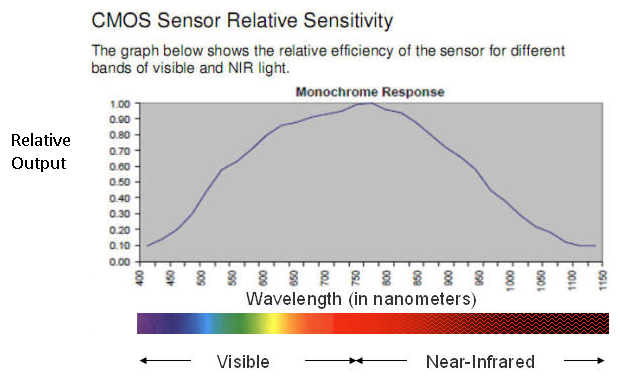
\includegraphics[scale=0.5]{../Figures/bandas}
\par\end{centering}

\protect\caption{Rango Espectral - mini-MCA\label{fig:Rango-Espectral--}}
\end{figure}


Para el caso espec�fico de la c�mara tetracam mini-MCA de 6 lentes
las bandas espectrales para cada lente est�n definidas as�: 490FS10-25
, 550FS10-25, 680FS10-25, 720FS10-25, 800FS10-25 , 900FS20-25, con
esta configuraci�n de lentes se abarca la mayor�a del espectro visible
e infrarrojo (Figura: \ref{fig:Rango-Espectral--} ). Cada imagen
debe ser corregida de deformaciones y sobrepuesta en un SIG que delimitar�
el �rea de estudio, as� se evitar� que ingrese informaci�n adicional
que dificulte el correcto an�lisis de informaci�n contenida en los
datos, esto permitir� realizar un an�lisis sobre cada lote productivo.

En campo se tomar�n muestras directas en los cultivos evaluados, con
la finalidad de realizar una calibraci�n del procedimiento de estimaci�n.
Esta calibraci�n se llevar� a cabo mediante la toma de informaci�n
de caracterizaci�n de suelos y principalmente de variables biof�sicas
y de poblaci�n que se desea estimar. Se realizar� un conteo manual
del n�mero de tallos mientras que en �reas peque�as al interior del
campo se realizara una muestra (destructiva) para el caso de la medici�n
de las variables biof�sicas. As�, con esta informaci�n de muestreo
ser� posible realizar un proceso de validaci�n cruzada junto a las
im�genes tomadas del campo lo que permita mejorar mucho m�s las estimaciones
finales realizadas a partir de las im�genes.

Lograr estimar la cantidad de toneladas de ca�a por hect�rea de manera
temprana es uno de los objetivos a nivel de industrial, en la teor�a
es posible estimar estas cantidades haciendo uso de las variables
biof�sicas y de poblaci�n antes se�aladas, pero en la pr�ctica no
se realiza, ya que algunas de las variables biof�sicas son medidas
mediante tomas de informaci�n de car�cter destructivo y con costos
elevados por lo cual no es posible hoy d�a.

En la actualidad se est� cambiando del paradigma de c�mo obtener la
informaci�n al referente a como almacenarla y analizarla adecuadamente.
Anteriormente la informaci�n se recolectaba mediante m�todos tradicionales
que no entregaban vol�menes de datos muy grandes, ahora se posee un
gran cantidad de sensores que pueden recolectar una cantidad inmensa
de informaci�n, la cual ser� la que alimentara nuestros modelos que
finalmente realizar� una aproximaci�n (modelaci�n) a los sucesos o
procesos naturales involucrados, esto con la necesidad de maximizar
los beneficios de dichos datos capturados. Dado este panorama hoy
en d�a existe una gama m�s amplia de algoritmos y m�todos estad�sticos
que permiten realizar un tratamiento y modelado de informaci�n m�s
amplio \citep{Mitchell:1997:ML:541177}. 

Es de gran importancia poder elegir con claridad cu�l es el m�todo
m�s adecuado en pro de la calidad de los resultados obtenidos del
procesamiento y modelado de la informaci�n, por lo cual se presenta
una metodolog�a general donde se nombran t�cnicas de gran inter�s
que podr�n ser evaluadas en el proceso de esta investigaci�n, a continuaci�n
se ve una propuesta anal�tica b�sica de c�mo se pretende abordar el
problema de investigaci�n.

\begin{figure}[H]
\centering{}\includegraphics[scale=0.7]{\string"C:/Users/SAMSUNG/Documents/GitHub/ProyectoMaestria/Final/Figures/Diagrama maestria (2)\string".png}\protect\caption{Propuesta Anal�tica B�sica}
\end{figure}



\subsubsection*{Flujo de procesos a realizar en esta investigaci�n:}

El insumo inicial para el desarrollo de este proyecto son las im�genes
multiespectrales tomadas sobre los cultivos de ca�a que se desean
evaluar, estas im�genes deben ser georeferenciadas y puestas sobre
un SIG una vez estas im�genes tienen estas caracter�sticas se proceder�
a realizaran los siguientes procesos sobre la informaci�n disponible:

~

Primero vamos a definir los sets de datos involucrados en el proceso
y que caracter�sticas est�n relacionadas a dichos datos:
\begin{enumerate}
\item Variables Iniciales

\begin{enumerate}
\item Usar los valores de las bandas espectrales de las im�genes como variables. 
\item Generar �ndices espectrales a partir de las bandas espectrales para
agregarlos como variables.
\item Recopilar informaci�n adicional tomada al principio del proyecto en
campo por ejemplo: Variables relacionadas a suelos y otras variables
medidas por muestreo que caractericen el �rea de estudio.\\
\begin{figure}[H]
\begin{centering}
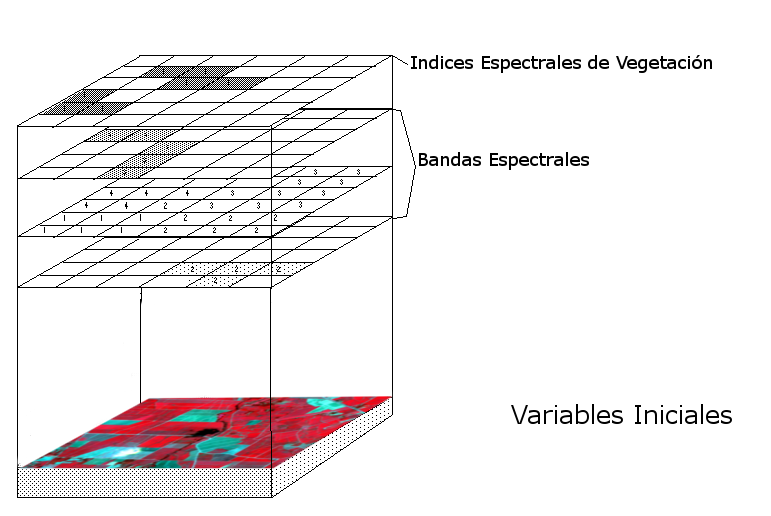
\includegraphics[scale=0.25]{../Figures/iniciales}
\par\end{centering}

\protect\caption{Variables Iniciales}
\end{figure}

\end{enumerate}
\item Variables Respuesta

\begin{enumerate}
\item Recopilar informaci�n de �rea Foliar e IAF por muestreo 
\item Recopilar informaci�n de cantidad de tallos por lote productivo\\
\begin{figure}[H]
\begin{centering}
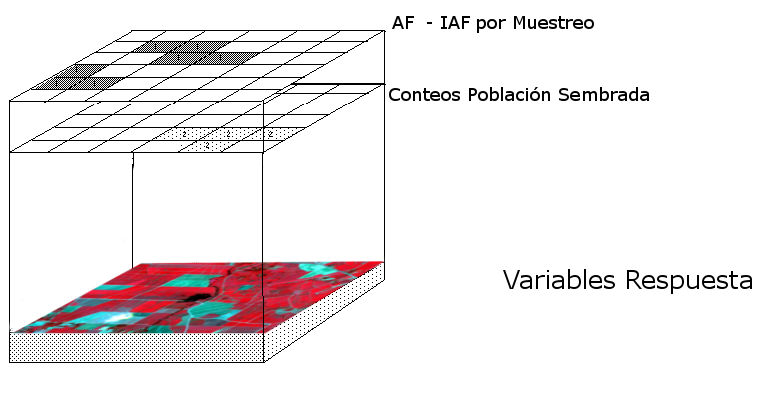
\includegraphics[scale=0.27]{../Figures/fianles}
\par\end{centering}

\protect\caption{Variables Respuesta}
\end{figure}

\end{enumerate}
\end{enumerate}
~

Con la informaci�n de las variables iniciales se realizaran los siguientes
procesos:
\begin{enumerate}
\item Estandarizar toda la informaci�n al tama�o de pixel adecuado para
maximizar la eficiencia del proceso y manejar la misma resoluci�n
espacial en todo el proceso.
\item Se realizar� un proceso de reducci�n de dimensionalidad considerando
distintos sets de variables. {[}Mediante An�lisis de Componentes Principales
\citep{Shlens05atutorial}{]} 
\item Realizar un proceso de clusterizaci�n o agrupamiento de pixeles con
caracter�sticas de respuesta espectral ajustando pixeles similares
a categor�a encontradas en los datos, donde dentro de cada clase se
minimiza la variabilidad y entre clases se maximiza la diferencia
entre estos. {[}Algoritmo K-medias \citep{Hartigan:1975:CA:540298}{]}.
\end{enumerate}
~

Con la informaci�n denominada variables respuesta se realizar� el
siguiente proceso:
\begin{enumerate}
\item Estandarizar toda la informaci�n al tama�o de pixel o resoluci�n a
igual escala a la tomada en los datos de variables iniciales.
\end{enumerate}
~

Despu�s de realizar estos procesos previos existen 2 posibilidades
para abordar el problema:
\begin{enumerate}
\item Usar solo los pixeles que tienen informaci�n tanto para las variables
iniciales como para las variables respuesta (depender� de la cantidad
de muestras tomados sobre el lote productivo) , con esta informaci�n
entrenar sistemas de aprendizaje o modelos estad�sticos.
\item Realizar una interpolaci�n en las variables respuesta a pixeles sin
informaci�n que contengan caracter�sticas de similar comportamiento
en la clasificaci�n de los datos iniciales (no depender� necesariamente
de la cantidad de muestras tomados sobre el lote productivo), con
esta informaci�n entrenar sistemas de aprendizaje o modelos estad�sticos.
\end{enumerate}
Cualquiera de los dos procesos tomados tendr� como resultado un modelo
de aproximaci�n a la respuesta de las variables biof�sicas o de poblaci�n
que se pretenden estimar, por lo cual es de gran importancia escoger
un adecuado proceso que permita registrar las estructuras de interacci�n
compleja en los datos de una forma adecuada.

La Regresi�n por m�nimos cuadrados parciales o PLS , Los Arboles Aleatorios
o Random Forest y el Aprendizaje por cuantificaci�n vectorial (LVQ)
son metodolog�as de un gran interes ya que una potencial aplicabilidad
desde la teor�a \citep{Breiman2001};\citep{hastie_09_elements-of.statistical-learning};\citep{Kohonen:1997:SM:261082},
pero se har� uso de aquel m�todo que entregue mejores resultados respecto
variables a estimar AF , IAF y NT, y se validara mediante un proceso
de validaci�n cruzada.

Una vez se han evaluado todas estas alternativas, se seleccionar�
el m�todo que permita realizar una mejor estimaci�n de las variables
biof�sicas y de cantidad poblacional o en su defecto una combinaci�n
de m�todos que mejore los resultados esperados, esta selecci�n se
realizar� mediante un proceso de validaci�n cruzada el cual consta
de dos subsets del total de los datos, donde uno de los subsets se
utiliza para entrenamiento del modelo evaluado y el otro para la validaci�n
del resultado obtenido mediante las im�genes multiespectrales en t�rminos
de la respuesta observada. La validaci�n cruzada o cross-validation
es una t�cnica utilizada para evaluar los resultados de un an�lisis
estad�stico y garantizar que son independientes de la partici�n entre
datos de entrenamiento y datos de prueba. Se utiliza en entornos donde
el objetivo principal es la predicci�n y se quiere estimar c�mo de
preciso es un modelo que se llevar� a cabo a la pr�ctica.\citep{Devyver1982}
Es una t�cnica muy utilizada en proyectos de inteligencia artificial
para validar modelos generados. 


\subsubsection*{Consideraciones respecto a la cantidad de informaci�n a ser procesada
en esta investigaci�n: }

Se considerar� una cantidad de im�genes de lotes productivos, que
sea muestreable tanto mediante toma de im�genes como de muestreadores
en campo, adem�s de considerar la capacidad de an�lisis de la informaci�n
muestreada. Por �ltimo, se evaluar� la resoluci�n final mediante la
cual se realizar� el an�lisis de los datos, esto se definir�a intentando
lograr un balance entre la ganancia en resoluci�n y la capacidad computacional
para realizar el procesamiento de los datos, con el prop�sito de asegurar
el pos-procesamiento de toda la informaci�n y extraer el m�ximo beneficio
de los datos adquiridos. Adem�s, dependiendo de la resoluci�n lograda
en las im�genes, es posible explorar metodolog�as de segmentaci�n
artificial sobre estas im�genes, que permita una mejor visualizaci�n
de las estructuras espaciales intr�nsecas presentes en los cultivos.



\section*{{\small{}Justificaci�n}}

{\small{}En Colombia los costos para producir una tonelada de az�car
son mayores que en otros pa�ses, a causa de m�ltiples factores como
el precio de la tierra, la mano de obra, los insumos, los impuestos,
la seguridad, el valor de los derechos de uso del agua, el costo de
fertilizantes e inclusive los costos de inspecciones para la detecci�n
de plagas y enfermedades. Igualmente, los recursos necesarios para
medir la sacarosa en la ca�a en evaluaciones de pre cosecha, y otros
rubros de importancia. Una manera de disminuir estos costos de producci�n
y mejorar la productividad de los campos es mediante la utilizaci�n
de herramientas para identificar las condiciones anormales en los
cultivos, de manera que se pueden tomar medidas de control o de prevenci�n
oportunas. El uso de percepci�n remota en combinaci�n con sistemas
de informaci�n geogr�fica (SIG) y sistemas de posicionamiento global
(GPS), generan una oportunidad para mejorar la competitividad de la
producci�n agr�cola asegurando el desarrollo sostenible de la actividad.}{\small \par}

{\small{}Las variables que se desean estimar por medio de esta metodolog�a
propuesta son de vital importancia para poder efectuar pron�sticos
tempranos de producci�n y sistemas de manejo sitio especifico en el
cultivo ca�a de az�car entre otras aplicaciones, lo que generar�a
avances importantes en el sector agro industrial de ca�a de az�car
en el Valle del Cauca relacionados a los siguientes factores:}{\small \par}
\begin{enumerate}
\item {\footnotesize{}Innovaci�n}{\footnotesize \par}

\begin{itemize}
\item {\footnotesize{}Actualmente no se utiliza fotograf�a a�rea para conocer
el estado del cultivo y tampoco se ha desarrollado algoritmos de inteligencia
artificial para vincular im�genes con la estimaci�n de par�metros
biof�sicos del cultivo.}{\footnotesize \par}
\end{itemize}
\item {\footnotesize{}Utilidad Econ�mica}{\footnotesize \par}

\begin{itemize}
\item {\footnotesize{}Actualmente se utilizan m�todos de medici�n sobre
cultivos de ca�a de az�car que conllevan altos costos econ�micos y
log�sticos.}{\footnotesize \par}
\end{itemize}
\item {\footnotesize{}Facilidad de aplicaci�n}{\footnotesize \par}

\begin{itemize}
\item {\footnotesize{}El sensor puede instalarse en plataformas a�reas,
como aviones de fumigacion, UAVs, gr�as u otros y la informaci�n puede
ser procesada facilmente una vez se establezca un protocolo estandar
resultante de esta investigaci�n.}{\footnotesize \par}
\end{itemize}
\item {\footnotesize{}Impacto ambiental}{\footnotesize \par}

\begin{itemize}
\item {\footnotesize{}Conocer el comportamiento del cultivo en una etapa
temprana (4 meses - 6 meses) donde se expresan caracter�sticas como
su crecimiento y desarrollo, permitir�a realizar tanto estimaciones
tempranas de producci�n como tambi�n evaluar el estado del cultivo.
Esto permitir�a realizar acciones de correcci�n cuando estas son necesarias,
logrando minimizar el impacto en costos y sobre el suelo, que se podr�an
producir si estas acciones se toman en una etapa posterior al periodo
de desarrollo del cultivo.}{\footnotesize \par}
\end{itemize}
\end{enumerate}


{\small{}Los ingenios tienen la necesidad de cuantificar el rendimiento
de los cultivos de ca�a de az�car, ya sea como un m�todo de seguimiento
del cultivo. Al lograr mejorar la resoluci�n de la toma de informaci�n
se enriquece mucho m�s el conocimiento del cultivo y as� puede llevar
a tener en cuenta pr�cticas realizadas sobre el cultivo que har�an
m�s preciso y menos emp�rico el manejo de los cultivos en pro del
rendimiento y calidad en la producci�n. }{\small \par}

{\small{}Realizar un proceso adecuado de estimaci�n de par�metros
biof�sicos en el cultivo de ca�a a partir de im�genes multiespectrales
genera una gran ganancia al estudio del comportamiento de la ca�a
a nivel de cultivo, adem�s de proveer informaci�n que hasta el momento
solo es capturada mediante costosos instrumentos, muchas veces necesariamente
estos procesos de medici�n deben ser destructivos. Adem�s logrando
capturar una mayor resoluci�n en im�genes multiespectrales unido a
sistemas de SIG es posible generar mapas mucho m�s detallados de importantes
caracter�sticas, tanto del cultivo como del comportamiento de los
suelos d�ndole un valor agregado a cada �rea estudiada.}{\small \par}


\subsubsection*{{\small{}Significado de la investigaci�n}}

{\small{}Se desea mostrar que el proceso de estimaci�n de caracter�sticas,
tanto de poblaci�n como biof�sicas, presente en cultivos de ca�a es
posible por medio del uso de im�genes multiespectrales y un correcto
procesamiento estad�stico de los datos mediante algoritmos no explorados
respecto a su aplicaci�n en cultivos de ca�a de az�car. Adem�s se
espera lograr la aplicabilidad real de este proceso de estimaci�n
para medir de forma no destructiva las variables biof�sicas, sobre
cultivos de ca�a que de otra manera no es posible. Adicionalmente,
se analizar� la factibilidad de implementar nuevas estrategias de
modelaci�n del cultivo y captura de datos para aprovechar al m�ximo
toda la informaci�n presente en el cultivo.}{\small \par}


\subsubsection*{{\small{}Facilidades Disponibles}}

{\small{}El trabajo se desarrollar� contando con informaci�n y datos
a portados por el programa de agronom�a del Centro de Investigaci�n
de la Ca�a de Az�car de Colombia y el �rea de biometr�a de esta entidad.
Los gastos adicionales distintos a la toma de informaci�n (computo,
papeler�a , etc.) ser�n solventados por el investigador.}


\pagebreak{}

\renewcommand{\refname}{}


\section*{{\normalsize{}Bibliograf�a}}

{\small{}\bibliographystyle{../Cites/apalike}
\bibliography{../Cites/bibliototal,\string"C:/Users/SAMSUNG/Desktop/Proyecto Maestria/Cites/bibliototal\string"}
}
\end{document}
